%
% This edited as https://www.overleaf.com/project/511e1f7f68f0b8591e232076
%
\documentclass[5p]{elsarticle} % use the 5p option to see in two columns

\usepackage{url}
\usepackage{amsmath}
\usepackage{amssymb}
\usepackage{hyperref}

\newcommand{\orcid}[1]{\href{https://orcid.org/#1}{\includegraphics[width=8pt]{orcid.png}}}

\journal{International Journal of Hydrogen Energy}

% This next bit patches the Elsevier ``Preprint submitted to.." footer
% on the first page
\makeatletter
\def\ps@pprintTitle{%
    \let\@oddhead\@empty
    \let\@evenhead\@empty
    \def\@oddfoot{\centerline{\hspace*{\fill} \raggedright DRAFT: \today} }%
    \let\@evenfoot\@oddfoot}
\makeatother
     
\begin{document}
\begin{frontmatter}


\bibliographystyle{elsarticle-num} % doesn't allow citet, but does format doi properly

\hyphenation{pipe-work}

\title{Low-pressure Hydrogen flow through the UK Gas Distribution Network \\ Supplementary Appendices}

\author[mjs]{Michael Sargent \orcid{0000-0001-9129-2990}\corref{cor1} }
\ead [mjs] {0000-0001-9129-2990}
\ead{michael.sargent@cambridgeenergy.uk}

\author[mjs]{Philip Sargent \orcid{0000-0002-1825-0097}}
\ead [pms] {0000-0002-0968-4467}
\ead{philip.sargent@cambridgeenergy.uk}

% \includegraphics[width=8pt]{orcid.png}
\cortext[cor1]{Corresponding author: Michael Sargent}
\address[mjs]{Cambridge Energy UK, 27 Greville Road, Cambridge CB1 3QJ, UK }


\hyphenation{pipe-work}
\end{frontmatter}

\appendix

\section{Software used in this study}
\label{sec:oursoftware}

The python code and input data is published on GitHub: \url{https://github.com/PhilipSargent/h2-in-pipes} under the MIT open source license\citep{Sargents_github}.

\section{Compressibility}
\label{appendix:gasprops}

All calculations in this paper have used an equation of state and  mixing rules appropriate to the pressure and temperature for each pure gas or blend studied. Individual corrections are small, but they multiply together to make a significant difference.

To calculate the compression factor as a function of temperature and pressure, and for gases such as natural gas composed of several different compounds, one needs an equation of state.
The low pressures and ambient temperatures of the distribution grid mean that several different equations of state are all sufficiently accurate.

Lozana $et$ $al.$ have recently reviewed\citep{Lozana2022}  the relevant equations of state and there are a bewildering variety of suitable functions.

 In this paper we use the 1978 Peng-Robinson equation of state\citep{Tabkhi2008, Abbas2021}, with temperature dependent binary interaction parameters and no volume translation corrections.
 For the exact calculation method used in this paper, see the code\citep{Sargents_github}. 

\section{Upgrading UK Boilers}
\label{appendix:more-boilers}

In the most recent English housing survey\citep{ehs21}, approximately one tenth (7/(59+7)) of domestic boilers on piped-gas were non-condensing and nine-tenths condensing: 
``the proportion of dwellings with a standard boiler decreased from 9\% in 2020 to 7\% in 2021, while the proportion with a condensing-combination boiler has increased from 57\% to 59\% in the same period".

However there are no statistics on how many of the condensing boilers have correctly-adjusted $50^\circ$C return-flow settings with appropriate weather compensation. Anecdotally, the proportion is very small, very likely less than 5\%. So a reasonable estimate would be that the return temperature is set to $50^\circ$C for 5\% of the condensing boilers and to $70^\circ$C for 95\% of them. There is no condensing for the non-condensing boilers so their efficiency is simply that at  a `condensation' temperature of $100^\circ$C.

We will assume
\begin{itemize}
    \item That 4\% of boilers are already perfectly adjusted, and the only change will be the multiplier of 0.974$\times$ from the change in fuel condensation behaviour
    \item That 86\% of boilers will go from a condensing temperature of $70^\circ$C (87.44\% with NG) to $50^\circ$C (93.69\% with hydrogen), a multiplier of  0.933$\times$
    \item That 10\% of boilers will change from an efficiency of  86.20\% (non condensing) to a fully-condensing, properly adjusted reflow temperature of 50$^\circ$C (93.69\% with hydrogen), a multiplier of 0.920$\times$
\end{itemize}
The population weighted efficiency multiplier is thus 0.933$\times$.

\subsection{Published boiler efficiencies}
Boiler efficiency\citep{Bennet2017} is measured either in a test rig at steady-state load, or estimated as a seasonal average as-installed in a house with a typical daily heating cycle and weather pattern. Repeated on- and off-periods increase losses\citep{saty2018}. 
Boiler manufacturer published efficiency values may be legally-required in some jurisdictions to be a seasonally-adjusted average number.

\section{Viscosities and temperature}
\label{sec:viscosities}

The viscosities of pure components are calculated from experimental data as a least-squares fit to a power law dependence on absolute temperature. 
Ideal gases have a power law relationship where the exponent is 0.5, the real gases here have exponents between 0.66 and 1.08. The viscosity of the gas mixture is a molecular fraction weighted average\citep{Krieger1951} of the viscosities of the components.

\begin{figure}[htb]
\centering
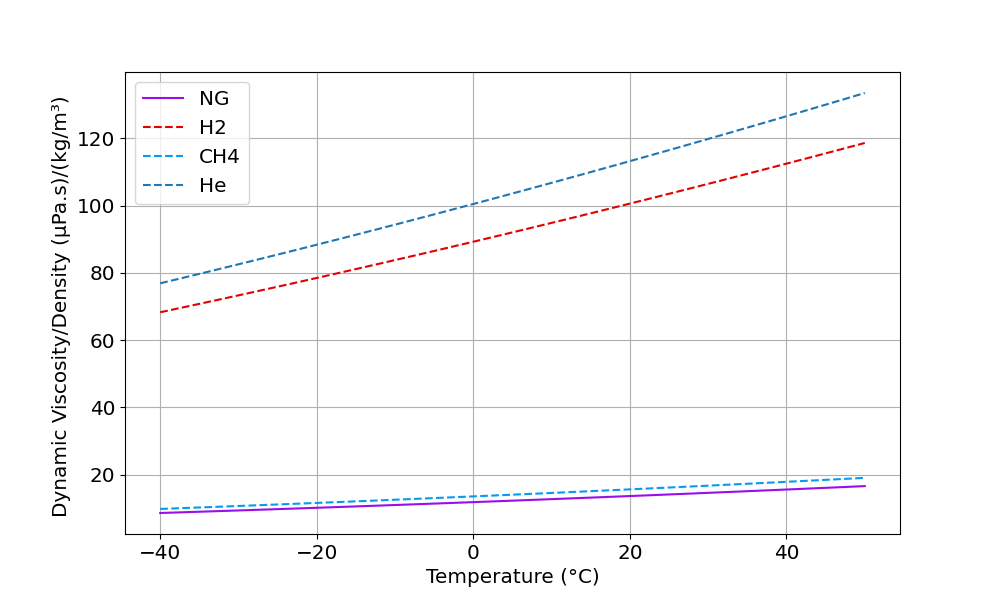
\includegraphics[width=0.49\textwidth]{peng_re.png}
\caption{Plot of kinematic viscosity: the ratio of dynamic viscosity and density, as a function of temperature at 1.06825 bar}
\label{fig:peng_re}
\end{figure}

Figure~\ref{fig:peng_re} shows the temperature dependence of the kinematic viscosities (the ratio of density to dynamic viscosity) of the natural gas blend, hydrogen and methane. This shows why it is important to do these calculations at a well-chosen reference temperature rather than using textbook values which may have been measured at a variety of different temperatures.

In the UK the ground temperature of the buried LP network is likely to stay in the range 5 to 15$^\circ$C all year\citep{MacKay2008}.

\subsection{The Blasius materials property}
\label{sec:blasiusparam}

Note that the term $\rho^{3/4} \cdot \mu^{1/4}$ in equation \eqref{eqn:pdrop0} is a materials' property which depends on temperature and pressure. We define this property as B, the Darcy-Weisbach Reynolds-Blasius parameter in equation \eqref{eqn:defnb}; or abbreviated to the 'Blasius parameter'.

\begin{equation}
\label{eqn:pdrop0}
\Delta P = \left ( \frac{4 \cdot 0.079}{D^{5/4}}\right ) \cdot \rho^{3/4} \cdot \mu^{1/4} \cdot v^{7/4}
\end{equation}

\begin{figure}[htb]
\centering
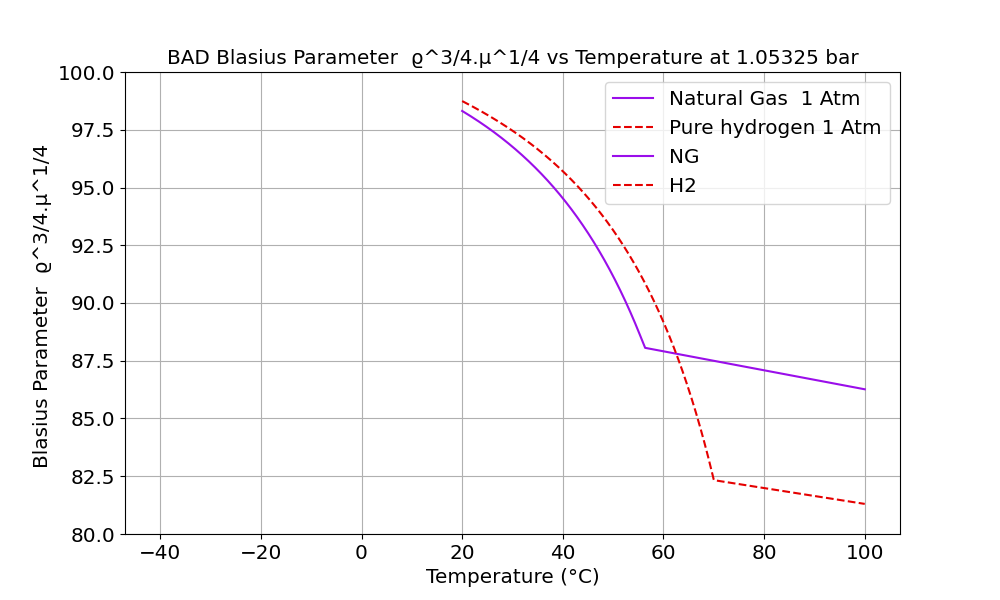
\includegraphics[width=0.49\textwidth]{peng_bf.png}
\caption{Blasius Parameter $\rho^{3/4} \cdot \mu^{1/4}$ ((kg/m)$\cdot$(m$\cdot$s)$^{-4}$ )}
\label{fig:blasiusparam0}
\end{figure}

\begin{equation}
\label{eqn:defnb}
B = \rho^{3/4} \cdot \mu^{1/4} 
\end{equation}
where $\rho$ is the density and $\mu$ is the dynamic viscosity.

Somewhat surprisingly, this materials' property has only a slight dependence on temperature as the dependencies of density and viscosity act in opposite directions. 

Also surprisingly, all the gases in the study have very similar dependence such that the normalised Blasius parameter, where the value for each gas is divided by the value for natural gas, is very nearly independent of temperature, varying less than 1.2\% between -40$^\circ$C and +50$^\circ$C.
%see Figure~\ref{fig:blasiusparam}.

%\begin{figure}[ht]
%\centering
%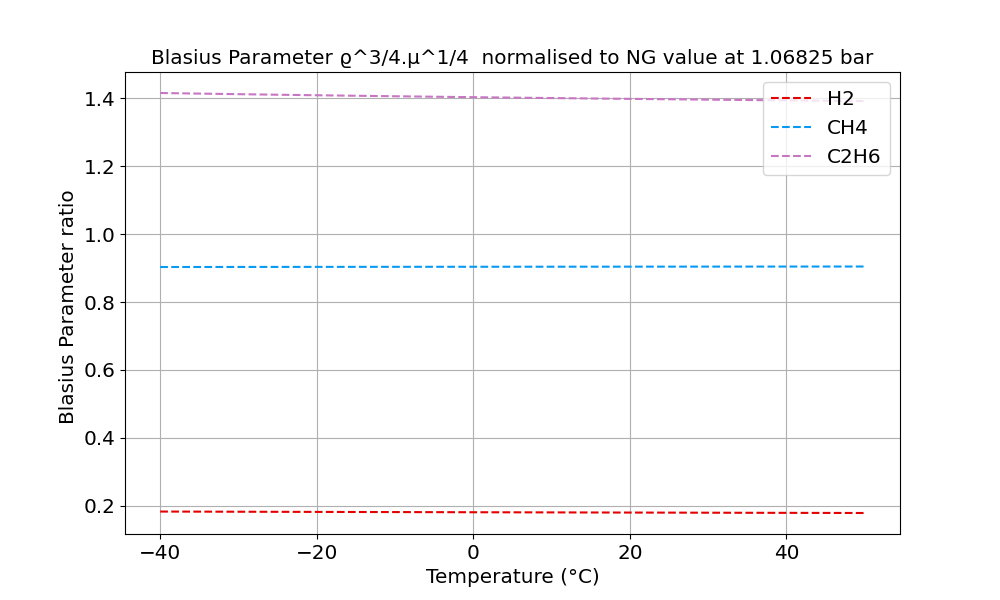
\includegraphics[width=0.49\textwidth]{peng_bf_NG.png}
%\caption{Ratio of Blasius Parameter to that of natural gas NG }
%\label{fig:blasiusparam}
%\end{figure}

This means that results calculated using the Blasius parameter, the relative pressure drop and the relative compression power requirement, are independent of temperature in the distribution grid.

\section{Dew point and partial pressure}
\label{sec:partial pressure}
Our calculations produce the partial pressure of water vapour in the flue gas, but we need the dew point. The two are related by standard tables of the saturation vapour pressure of water\citep{Perry2008}: the pressure at which water vapour is in thermodynamic equilibrium with its condensed state.

The range of atmospheric pressure in the UK means that the dew point of the flue gas varies  $\pm1.4^\circ$C, which affects the maximum efficiency.

\section{The Peng-Robinson calculations}

Equations of state for gas mixtures are still an active research area\citep{Lozana2022} and there is continual development of alpha functions, interaction parameters and mixing rules e.g. Pina-Martinez $et$ $al.$\citep{Pina-Martinez2019}.

\subsection{Calculating the properties of a gas mixture}
\label{sec:gasmix}
The higher heat capacity and the mean molecular weight of the Fordoun natural gas are calculated from a mole fraction weighted sum of those properties of the component pure gases.

The compressibility and density of the natural gas are calculated for a given temperature and pressure using the Peng-Robinson equation of state: 

\begin{enumerate}
\item The Peng-Robinson\citep{Pina-Martinez2019} parameters $a$ (attraction) and $b$ (repulsion) for each pure component at a given temperature are calculated from the critical temperature $T_c$, the critical pressure $P_c$, and the $omega$ coefficient (a measure of the molecule asphericity) of each pure gas.
    \item the coefficient $b$ of the mix is  the weighted sum of the $b$ values of the component gases, where the weights are the mole fractions. 
    \item The temperature dependent binary interaction parameter k is calculated using the Courtinho method~\cite{Privat2023} from the $b$ value of each gas in a pair. For an 11 component gas there are 55 pairwise interactions.
    \item The $a$ values are calculated as the weighted sums of the geometric means of the pair-wise values of $a$ between each pair of components. The weights are the mole factions of each pair multiplied together, times the value (1-$k$)
    \item The effective $T_c$, $P_c$ and $omega$ of the natural gas, the pseudo-component,  are calculated from the $a$ and $b$ values for the mix for the given temperature
    \item the compressibility and thus the density of the natural gas is calculated using the effective $T_c$, $P_c$ and $omega$ values.
\end{enumerate}
The precise algorithm is in the code on GitHub~\cite{Sargents_github}.
\section{References}
\bibliography{h2pipe}

\end{document}